
% Proposta TCC1 - Professora Ana Cristina B. Kochem Vendramin (cristina@dainf.ct.utfpr.edu.br, criskochem@utfpr.edu.br)

\documentclass{normas-utf-tex_07_2012} %Estilo de Formato criado pelo Prof. Hugo Vieira Neto (hvieir@utfpr.edu.br)
%Se você ainda não conhece o latex, comece olhando o site do Prof. Hugo --> http://pessoal.utfpr.edu.br/hvieir/orient/

%\documentclass[twoside,openright]{normas-utf-tex} %openright = o capitulo comeca sempre em paginas impares

\usepackage[alf,abnt-emphasize=bf,bibjustif,recuo=0cm, abnt-etal-cite=2, abnt-etal-list=99]{abntcite} %configuracao das referencias bibliograficas.
\usepackage[brazil]{babel} % pacote portugues brasileiro
\usepackage[utf8]{inputenc} % pacote para acentuacao direta
\usepackage{amsmath,amsfonts,amssymb} % pacote matematico
\usepackage[pdftex]{graphicx} % pacote grafico
\usepackage{times} % fonte times
\usepackage{a4wide}
\usepackage[a4paper]{geometry} %define papel a4...
\geometry{left=3cm,right=2cm,top=3cm,bottom=2cm} % ...e suas margens
\usepackage{tabularx,multirow,longtable} %pacotes para mesclar linhas/colunas; tabelas grandes
\usepackage{fancyhdr} % altera cabeçalhos
\usepackage[T1]{fontenc} % acentuação direto no texto
\usepackage{ae} % “Almost European”: aumenta a qualidade do pdf final
\usepackage{rotating} % faz rotações de tabelas e figuras
\usepackage{indentfirst} % tabula a primeira linha do parágrafo
\usepackage[hang,small,bf]{caption} % legendas; nome "tabela" ou "figura" em negrito
\usepackage{caption3}
\usepackage{setspace} % ajuste do espaço entre-linhas
\usepackage{algorithm}
\usepackage{subfig}
\usepackage{float} % posicionamento das figuras
\usepackage{subfloat}
\usepackage{arydshln}
\usepackage{enumitem}
\makeatletter
\renewcommand{\ALG@name}{Algoritmo}
\usepackage{algorithmic}

%Italico e negrito customizados (\it e \bf)
\renewcommand{\it}[1]{\textit{#1}}
\renewcommand{\bf}[1]{\textbf{#1}}

%para a hifenacao funcionar é necessario fazer a seguinte modificacao
%Clique em Iniciar -> Programas -> MikTeX -> MiKTeX options Vá em Languages e marque a caixa português.

%hifenacoes customizadas
\hyphenation{mo-de-lar re-no-vá-veis re-pre-sen-tar re-pre-sen-ta-ção la-te-rais res-pec-ti-vos re-a-ção re-a-li-zan-do o-pe-ra-ções cons-tan-te di-fe-ren-tes tem-pe-ra-tu-ra ex-tre-mi-da-de ter-mo-di-nâ-mi-ca trans-es-te-ri-fi-ca-ção In-ter-net}

%%%% Comandos introduzidos para controlar as alteracoes no fonte%%%%%%%%%%%%%%%%%
% assigning colors to comments of each author
\usepackage{color}
\newcommand{\cris}[1]{\textcolor{blue}{#1}} %texto final
\newcommand{\crisC}[1]{[\textcolor{blue}{#1}]} % comentário entre colchetes
%%%%%%%%%%%%%%%%%%%%%%%%%%%%%%%%%%%%%%%%%%%%%%%%%%%%%%%%%%%%%%%%%%%%%%%%%%%%%%%%%%%%%%

% ---------- Preambulo ----------
\instituicao{Universidade Tecnol\'ogica Federal do Paran\'a} % nome da instituicao
\programa{Departamento Acad\^emico de Inform\'atica} % nome do programa ou departamento
\area{Curso de Engenharia de Computa\c{c}\~ao} % área ou curso

\documento{APS} % [Trabalho de Conclus\~ao de Curso] ou [Disserta\c{c}\~ao] ou [Tese]
\nivel{Gradua\c{c}\~ao} % [Gradua\c{c}\~ao], [Especializa\c{c}\~ao], [Mestrado] ou [Doutorado]
\titulacao{Engenheiro} % [Engenheiro], [Tecn\'ologo], [Bacharel], [Mestre] ou [Doutor]

\titulo{\MakeUppercase{Documento de projeto}} % titulo do trabalho em portugues
\title{\MakeUppercase{}} % titulo do trabalho em ingles

\autor{Marcelo Teider Lopes} % autor do trabalho
\autordois{Stefan Campana Fuchs}
% \cita{SOBRENOME, Nome Autor} % sobrenome (maiusculas), nome do autor do trabalho

\palavraschave{Incluir as palavras-chave em português} %substituir pelas palavras-chave relacionadas ao seu tema de pesquisa
\keywords{Incluir as palavras-chave em inglês} % incluir palavras-chave em inglês

\comentario{\UTFPRdocumentodata\ de Sistemas Embarcados apresentada ao \UTFPRprogramadata\ da \ABNTinstituicaodata\ como requisito parcial para obten\c{c}\~ao dos títulos de ``Bacharel em Sistemas de Informação'' e ``Engenheiro em Computa\c{c}\~ao''.} %\\ \'Area de Concentra\c{c}\~ao: \UTFPRareadata.}

\orientador{Prof. Douglas Paulo Bertrand Renaux} % <- no caso de orientadora, usar esta sintaxe
% \coorientador[Co-orientadora:~]{~} % <- no caso de co-orientadora, usar esta sintaxe

\local{Curitiba} % cidade
\data{2014} % ano

\setcounter{tocdepth}{4} % para numeração das seções
\setcounter{secnumdepth}{4}

\numberwithin{equation}{chapter} %
%\numberwithin{table}{chapter} %
%\numberwithin{figure}{chapter} %

\makeatletter  %% this is crucial
 \renewcommand\subsubsection{\@startsection{subsubsection}{3}{\z@}%
                        {-2\p@ \@plus -0.5\p@ \@minus -0.5\p@}%
                        %{8\p@ \@plus 4\p@ \@minus 4\p@}%     <-- this is copied from the subsection command
                        {2\p@ \@plus 1\p@ \@minus 1\p@}%     <-- this is copied from the subsection command
                        {\normalfont\normalsize\bfseries\boldmath
                         \rightskip=\z@ \@plus 8em
 \pretolerance=10000 }}
\makeatother   %% this is crucial

%---------- Inicio do Documento ----------
\begin{document}

\capa % geracao automatica da capa

\folhaderosto % geracao automatica da folha de rosto

% dedicatória (opcional)
%\begin{dedicatoria}
% Texto da dedicat\'oria.
%\end{dedicatoria}

% agradecimentos (opcional)
%\begin{agradecimentos}
% Texto dos agradecimentos.
%\end{agradecimentos}

% epigrafe (opcional)
%\begin{epigrafe}
%\end{epigrafe}

% %resumo
% \begin{resumo}
% 
% 
% Incluir o resumo aqui
% 
% 
% \end{resumo}
% 
% %abstract
% \begin{abstract}
% 
% 
% Include the abstract here
% 
% 
% \end{abstract}

% listas que recomenda-se a partir de 5 elementos
\listadefiguras % geracao automatica da lista de figuras
%Elaborado de acordo com a ordem apresentada no texto, com cada item designado por seu nome específico, acompanhado do respectivo número da página.

%\listadetabelas % geracao automatica da lista de tabelas
%Elaborado de acordo com a ordem apresentada no texto, com cada item designado por seu nome específico, acompanhado do respectivo número da página.

%\listadesiglas % geracao automatica da lista de siglas
%Constituída de uma relação alfabética das abreviaturas e siglas utilizadas no texto, seguido das palavras ou expressões correspondentes grafadas por extenso. Utilizada apenas se houver siglas.

%\listadesimbolos % geracao automatica da lista de simbolos
%Elaborado de acordo com a ordem apresentada no texto, seguido do significado correspondente. Utilizada apenas se houver símbolos.

% sumario
\sumario % geracao automatica do sumario

%---------- Inicio do Texto ----------

\setcounter{page}{4} % *** Necessário arrumar manualmente antes de imprimir

% Recomendo a criação de um arquivo .tex para cada capítulo do seu trabalho. Isso facilitará, principalmente, quando vários usuários estiverem editando o mesmo documento.
% Neste momento, colocarei tudo aqui no mesmo .tex.
% Para usar arquivos diferentes, basta descomentar os comandos abaixo.
%\input{Introducao.tex}
%\input{LevantamentoBibiografico.tex}
%\input{Metodologia.tex}
%\input{Recursos.tex}
%\input{Viabilidade.tex}
%\input{Contexto.tex}
%\input{Conclusao.tex}

% Criando o capítulo Introdução. Caso crie um arquivo .tex, basta inserir o texto abaixo dentro do arquivo.
% O label serve para referenciar o capítulo quando necessário
\chapter{Arquitetura funcional}

O diagrama da Figura \ref{fig:arq_funcional} expôe uma representação da arquitetura funcional do sistema. As setas representam o sentido dos fluxos de dados entre cada função do sistema. 

``Comunicação com o computador'' envolve a UART (física e driver), e o protocolo de comunicação do sistema. Esta função é utilizada para a comunicação com o simulador de elevador, que é executada em um computador. ``Recebe entrada dos botões'' recebe requisições dos botões internos e externos de andares, feitas pelos usuários do elevador. A função ``Controla luzes dos botões'' é responsável por ligar ou desligar as luzes dos botões de acordo com as requisições recebidas dos usuários e de acordo com o movimento do elevador. ``Enfileira requisições'' é responsável por organizar as requisições de botões na ordem em que devem ser atendidas. ``Controla movimento das portas'' efetua a abertura e fechamento das portas, de acordo com a lógica de funcionamento do elevador. ``Controla movimento do elevador'' é responsável por fazer o elevador subir ou descer para atender às requisições enfileiradas.

\begin{figure}[h]
    \centering
    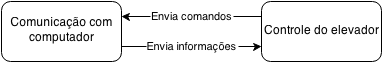
\includegraphics[width=0.8\columnwidth]{./figures/arq_funcional.png}
    \caption{Diagrama da arquitetura funcional do sistema.}
    \label{fig:arq_funcional}
\end{figure}

\section{Alocação das funções em Hardware e Software}

\begin{table}[h!]
\caption{Alocação das funções em Hardware e Software.}
\centering
\begin{tabular}{|c|c|c|}
\hline
\textbf{Bloco} &\textbf{Hardware} & \textbf{Software} \\ \hline \hline
Comunicação com o computador & X & X \\
Recebe entrada dos botões & - & X \\
Controla luzes dos botões & - & X \\
Enfileira requisições & - & X \\
Controla movimento das portas & - & X \\
Controla movimento do elevador & - & X \\
\hline
\end{tabular}
\label{tab:publicacao}
\end{table}

A função de comunicação com o computador constitui-se tanto de hardware quanto de software. A parte de hardware está relacionada ao periférico UART0 do Kit LPC1768. O software relaciona-se ao driver desenvolvido para inicializar e utilizar este periférico, além do protocolo de comunicação do sistema.

O restante das funções é constituida apenas de software, pois controlam a lógica de operação do sistema, não fazendo diretamente o uso de periféricos.






\chapter{Arquitetura física}

\section{Uso de memória}

A Tabela \ref{tab:uso_memoria} apresenta o uso estimado das memórias RAM e flash do Kit LPC1768 para o desenvolvimento do sistema. Considerou-se na estimativa apenas os componentes que já estavam disponíveis ao projeto anteriormente (CMSIS RTOS e driver da UART). Pela análise, como a maior parte das memórias permanece livre, considera-se que a quantidade é suficiente para o desenvolvimento dos componentes restantes do sistema.

\begin{table}[h!]
	\caption{Uso estimado das memórias do Kit LPC1768.}
	\centering
	\begin{tabular}{|c|c|c|}
		\hline
		\textbf{} &\textbf{RAM (64 kB máx.)} & \textbf{Flash (512 kB máx.)} \\ \hline \hline
		CMSIS RTOS & 2600 B & 5400 B\\
		Driver da UART & 150 B & 800 B\\
		\hline
		\bf{Total ocupado} & 2750 B (2.68 kB) & 6200 B (6.05 kB)\\
		\bf{Total Livre} & 61.32 kB (95.81\%) & 505.95 kB (98.82\%) \\
		\hline
	\end{tabular}
	\label{tab:uso_memoria}
\end{table}


\section{Diagrama de objetos}



\section{Projeto dos componentes}

A Figura \ref{fig:maq_estados} apresenta um diagrama de estados, contendo a visão geral do funcionamento do sistema. O estado ``Inicialização'' compreende todas as funções que são necessárias para iniciar a operação do sistema (como por exemplo, inicializar o driver da UART, sistema operacional, variáveis internas, entre outros). O estado ``Ocioso'' representa a situação em que o elevador não possui requisições pendentes, sendo que neste caso ele permanece parado no mesmo andar e com as portas abertas. 

Os estados ``Subindo'' e ``Descendo'' são muito similares internamente, ambos representado situações em que o elevador está atendendo a requisições de usuários. A diferença está essencialmente na direção de movimento do elevador. Os seus sub-estados especificam o modo de operação do elevador para atender às demandas de deslocamento até os andares requisitados. Todas as requisições de usuários são enfileiradas por prioridade, em uma tarefa separada (enfileirador). O próximo andar que o elevador deve ir fica sempre no topo da fila, sendo que as a maioria das decisões e transições nos estados e sub-estados depende de qual é este andar.

A comunicação com o computador (executanto a simulação de elevador) está presente de forma implícita no diagrama, o que inclui o recebimento de requisições de botões, recebimento de informações de posição do elevador e envio de comandos ao elevador e portas.

\begin{figure}[h]
    \centering
    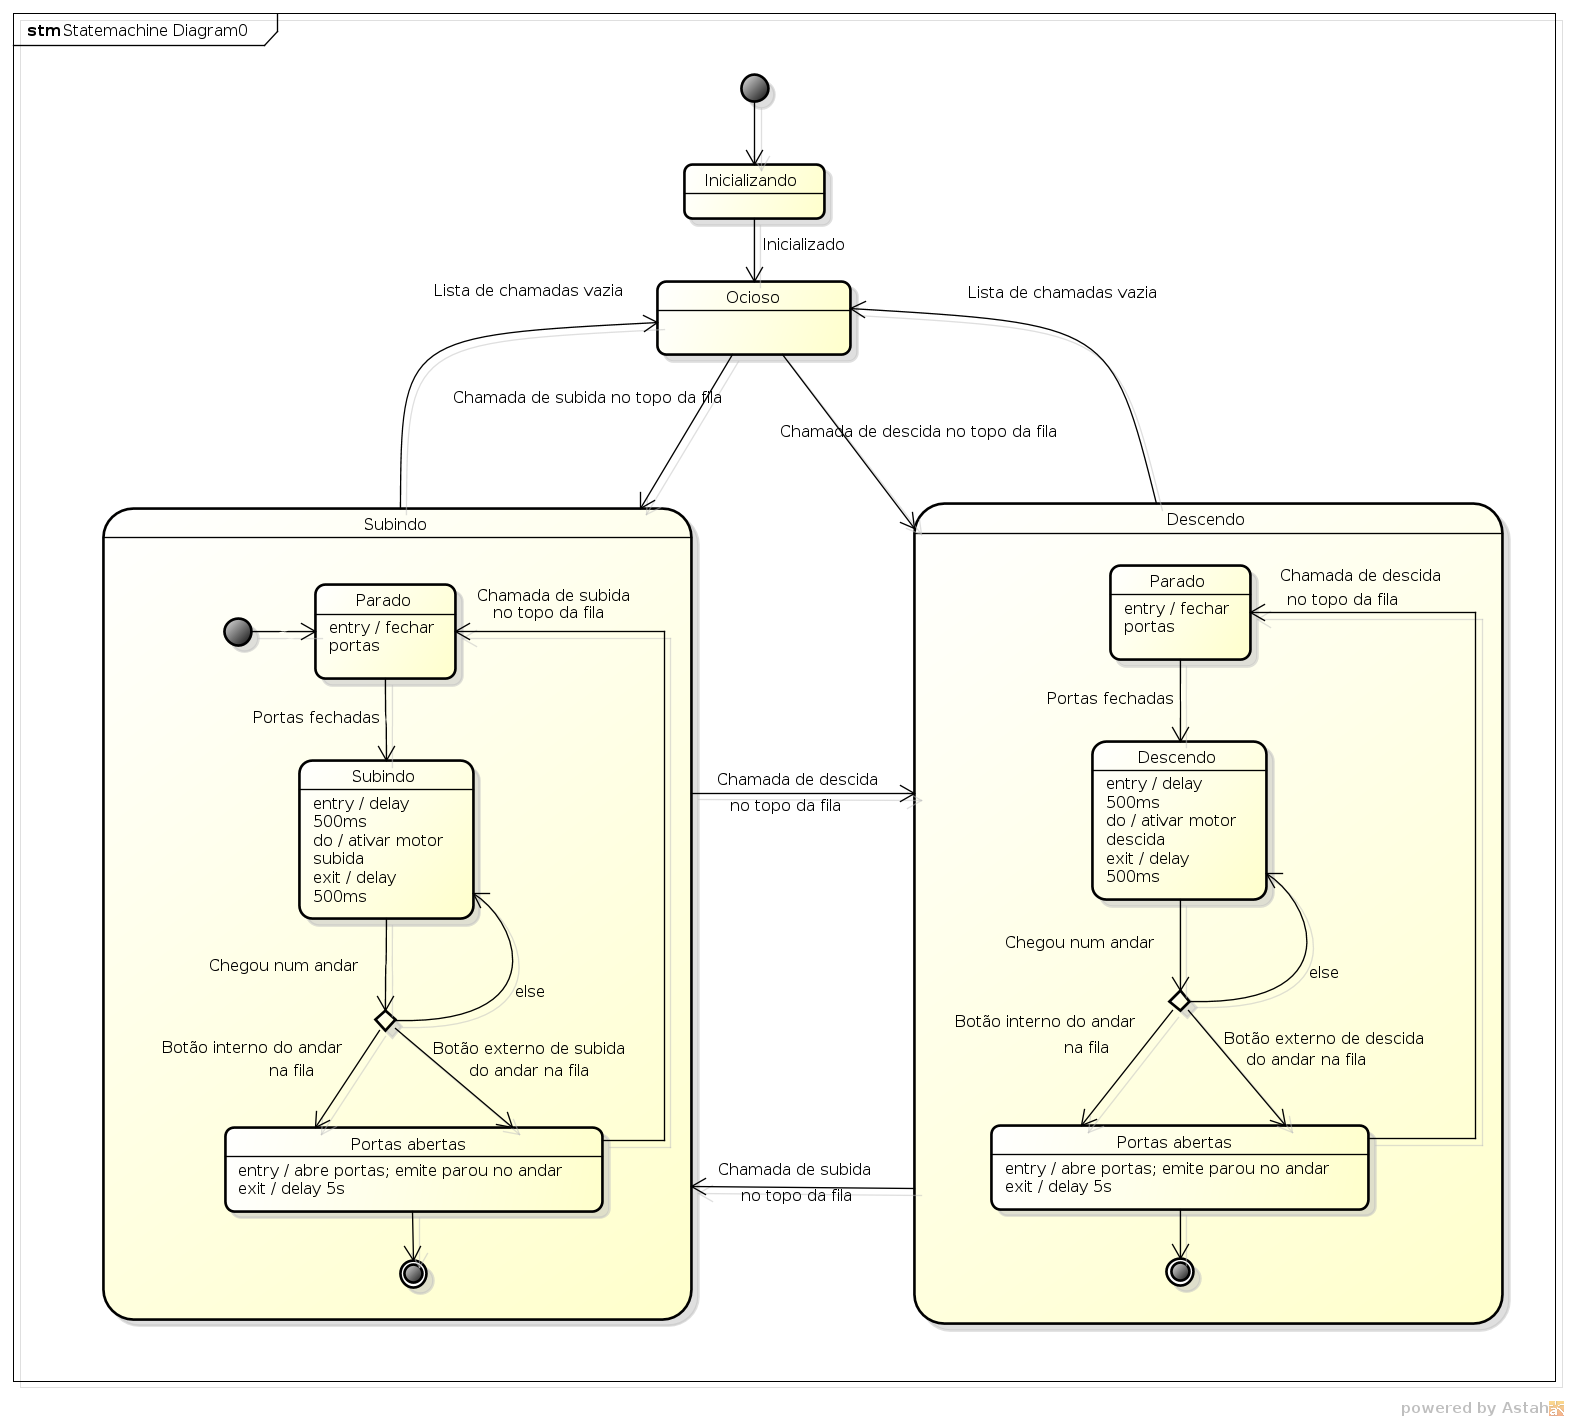
\includegraphics[width=1\columnwidth]{./figures/maq_estados.png}
    \caption{Diagrama de estados geral do sistema.}
    \label{fig:maq_estados}
\end{figure}





% \chapter{Projeto dos componentes}

\begin{itemize}
	\item UART: já presente no Kit LPC1768;
	\item Driver UART: implementado anteriormente, seguindo o especificado em estudo da plataforma;
	\item ISR UART: implementado em conjunto com o driver da UART;
	\item Buffer UART: implementado em conjunto com o driver da UART;
	\item Controlador do elevador: Monitora constantemente os sensores do elevador, e envia comandos aos atuadores de acordo com a lógica de operação do elevador. 
	\item Protocolo de comunicação: Recebe informações do buffer da UART, interpreta o seu significado e repassa-as para a função de tratamento do controlador do elevador; Recebe comandos do controlador, converte-os para uma linguagem aceita pelo simulador e repassa-os para o buffer da UART.
\end{itemize}






%---------- Referencias ----------

% \chapter{Referências Bibliográficas}

% \nocite{sumo_overview} %remover depois, está aqui só para conseguir compilar (precisa ter pelo menos 1 referencia)!
% \bibliography{Referencias}

%---------- Apêndices e Anexos ----------
% % Apêndice
% \appendix
% %\input{Apendice.tex} % Para criar um arquivo separado para o Apêndice, descomente essa linha e comente a linha abaixo
% \chapter{Título do Apêndice}
% 
% % Anexo
% \appendix
% \renewcommand{\appendixname}{Anexo} % Para criar Anexo ao invés de Apêndice
% %\input{Anexo.tex} % Para criar um arquivo separado para o Anexo, descomente essa linha e comente a linha abaixo
% \chapter{Título do Anexo}

\end{document}
